

\section{Tubo de Silicone e Cola de Silicone}
\label{borracha}


\begin{table}[ht!]

	\begin{tabular}{r l|l p{12cm} }
		
		\textcolor{gray}{Especificação} &&& 	{Tubo Silicone e Cola Silicone
		Incolor}\\
		\textcolor{gray}{Data} &&& 				{31/05/2014}\\
        \textcolor{gray}{Beneficiado} &&&		{Mercado da Borracha} \\
        \textcolor{gray}{CNPJ} &&& 				{05.245.187/0001-07} \\
        \textcolor{gray}{Número Nota} &&& 		{23827} \\
		\textcolor{gray}{Quantidade} &&& 		{-} \\
		\textcolor{gray}{Valor} &&& 			{R\$73,00} \\
		\textcolor{gray}{Data Sheet} &&& 		{-} \\

		\textcolor{gray}{Função no projeto} &&& {Os tubos e colas de silicone são
		utilizados nas emendas de cabos submarinos.}
		\\
		\textcolor{gray}{Razão da Escolha} &&& {-}
		

	\end{tabular}
\end{table}

\newpage

\subsection{Nota Fiscal}
\begin{figure}[H]
 \centering
 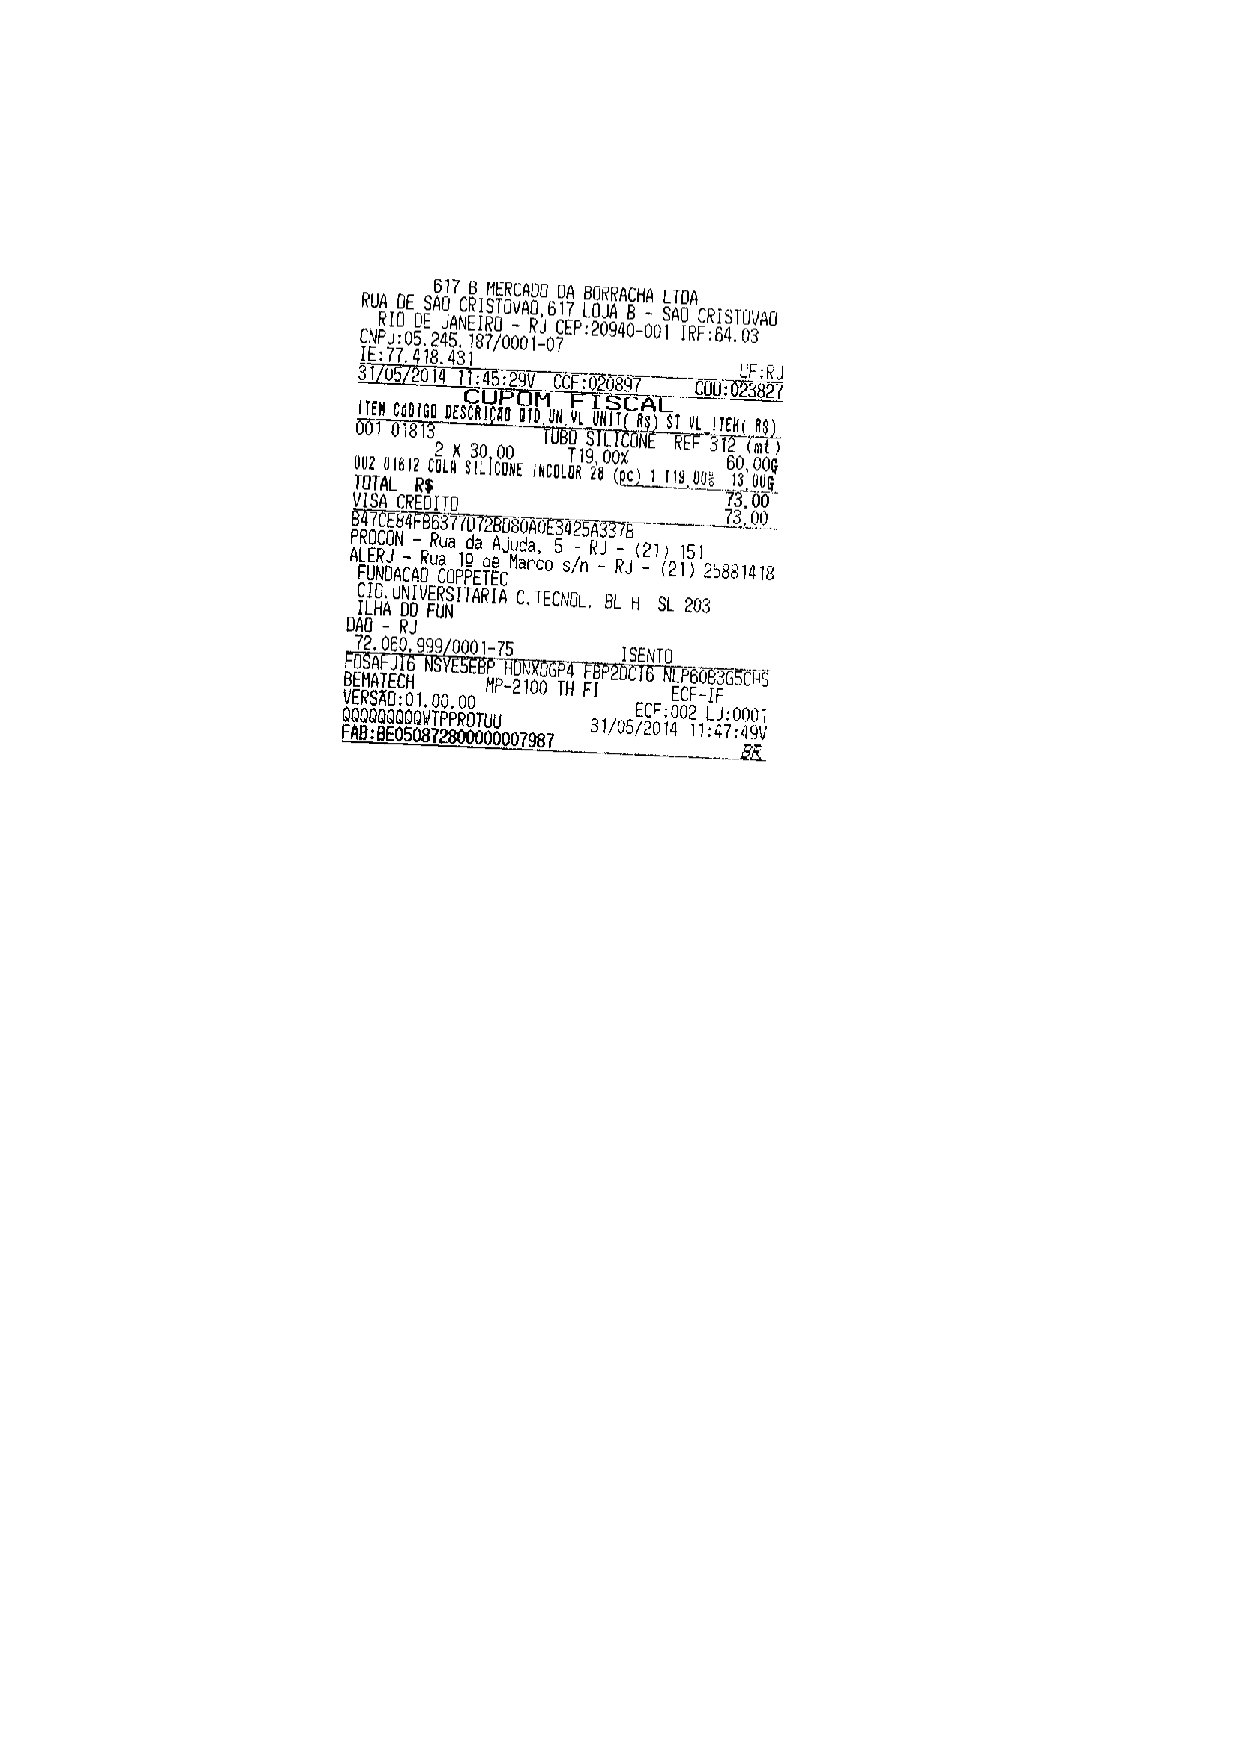
\includegraphics[width=1\columnwidth]{Borracha/nota_borracha.pdf}
 \caption{Tubo e cola de silicone}
 \end{figure} 